% !TeX root = ../thuthesis-example.tex

\chapter{集群故障检测}

本章节描述了高可用优化下的集群错误检测机制。ConfigNode Leader 是集群故障检测的负责人。ConfigNode Leader通过维护和DataNode之间定期心跳的方式来获取每个节点的基本负载情况、Region负载情况等信息,通过定期要求DataNode之间进行P2P探测的方式来获取集群的网络拓扑结构。同时,我们使用了基于Phi Accural的检测算法对于收集到的探测包进行故障研判,并根据Thrift进行了一些优化。

\section{节点和Region的心跳机制}

IoTDB使用心跳机制来探测集群内部节点和每一个Region的健康状态,从而能够第一时间检测出集群内进程崩溃、网络分区的问题。

ConfigNode是集群的大脑,负责维护每一个节点的状态信息。在ConfigNode、DataNode和AINode启动的时候,都需要向ConfigNode的Leader汇报自己的启动信息,由ConfigNode Leader将其纳入心跳管理的范围内。当节点下线、被移出集群、重启时也会汇报最新的状态,让ConfigNode Leader知悉。

对于注册在集群的所有节点,ConfigNode会定期使用内部RPC向每一个节点发送心跳,来更新确认节点的最新状态。心跳会按照固定时间间隔触发,通常间隔是1s。
ConfigNode Leader会通过心跳向DataNode传输Quota和集群拓扑结构等信息,

DataNode会通过心跳上报当前的状态、节点的CPU、内存、磁盘的使用情况、每一个Region目前的Consensus的Leader分布、每一个Region的磁盘使用情况、日志同步情况、当前的Pipe任务情况等相关内容。


在收集到心跳样本之后,ConfigNode Leader会根据心跳样本的情况对集群的情况做出处理。

ConfigNode首先会对该节点本本身的状态进行研判。在2.0.2.1等先前版本中,如果在一个固定的超时间隔之内(通常是20s)都没有收到DataNode上报的心跳,那么ConfigNode Leader就会研判该节点已经失效,将该节点的状态从RUNNING标记为UNKNOWN。这种基于固定超时时间间隔的算法能够检测出大部分的实际问题,但依然有改进的空间,再下一个小节中我们通过提出基于PhiAccrual的方式对该研判方法进行升级。

ConfigNode其次会根据收集到的Load情况和每一个Region的情况进行相应的研判,从而做出预防性高可用的操作。例如负载均衡、Region迁移、磁盘告警等操作,从而减少错误的产生。


(这部分可以增加一张示意图来描述整一个过程)
(这部分可以详细描述预防性操作的一些行为)



\section{基于Phi Accrual的故障检测}

如前文所述,在2.0.2.1等先前版本之前,ConfigNode Leader采用基于心跳的固定超时来研判节点的存活情况。该算法研判的核心参数在于超时时间 $\Delta_{t}$,即当ConfigNode Leader在超过 $\Delta_{t}$ 的时间内没有收到DataNode的心跳包,则会认为该节点宕机。

参数 $\Delta_{t}$ 是故障检测的检测速度和检测正确度的权衡。如果 $\Delta_{t}$ 很短,那么节点故障会被快速发现,但对应的误报率就会很高。如果$\Delta_{t}$很长,那么误报率就会对应下降,但是代价就是错误的平均发现时间变长。

这种基于心跳的固定超时算法的优点在于逻辑简单直接,易于实现和部署,并且在IoTDB已有的实践中能胜任大部分的错误发现。然而这种算法依然存在诸多问题。
首先,$\Delta_{t}$ 参数的选择需要人工介入,需要对业务集群的特性有所了解,对很多用户来说是一个很大的心智负担。其次,$\Delta_{t}$ 参数一旦确定,轻易不能改变,这导致心跳算法无法对集群随时间的状态迁移作出适配。例如,集群流量如果有明显的时段性变化,那么显然在高负载时期和低负载时期都使用同一个参数并不明智。最后,该算法只能给出故障/正常的二元结论,无法给出量化的数据。

前文提出的Phi Accural算法有冷启动的问题。因此我们的故障检测综合

1. 冷启动阶段。在集群刚启动,尚未收集足够的心跳样本的时候,我们使用基于心跳的固定超时来负责初始时期的节点存活判断,同时收集这些样本。当我们收集了足够的样本数量(默认为60个)的时候,我们切换成基于Phi Accural的算法来研判节点的存活率。

1. 心跳历史样本收集。检测器会收集每一个DataNode心跳包,并计算出连续两个心跳包之间的间隔,并存储在一个固定大小的采样窗口内,当有新的心跳包到达的时候,最新的时间间隔会被存入采样窗口,而最早期的第一个数据将会被删除。

2. 根据采样窗口计算到达间隔的分布,并计算 $\phi$ 值。我们将到达间隔认为是符合正态分布。那么我们就可以从采样窗口来估计这个分布的均值 $\mu$ 和方差 $\sigma^2$。那么,在上一次心跳到达t时间之后才会有下一次心跳到达的概率可以通过下列公式计算出来:

$$ P_{later}(t) = \frac{1}{\sigma\sqrt{2\pi}} \int_{t}^{\infty} e^{-\frac{(x-u)^2}{2\sigma^2}} dx $$

3. 计算 $\phi$ 并根据设定阈值进行比较。我们使用如下的公式进行定义:

$$ \phi(now) = -log_{10}(P_{later}(t_{now} - t_{last})) $$

不同的阈值代表着本次研判出错的概率。阈值=1的时候研判出错的概率是10\%,阈值=1的时候研判出错的概率是1\%,阈值=3的时候研判出错的概率是0.1\%。

「在实验章节给出这两种故障检测算法的实验对比」

\section{集群网络拓扑感知}

上述所述的心跳和故障检测机制能够迅速识别集群中的节点宕机和对称性网络分区等问题,但针对非对称网络分区等问题依然无法识别。为此,我们需要在此基础上增加集群网络拓扑感知能力。

\begin{figure}
  \centering
  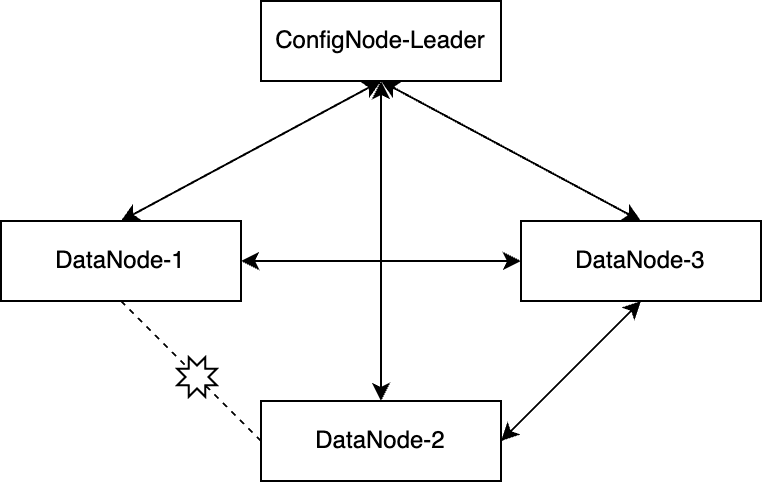
\includegraphics[width=0.9\linewidth]{c03-parition.png}
  \caption{系统非对称分区示意图}
  \label{fig:c03-partition}
\end{figure}

考虑图\ref{fig:c03-partition}所示的系统情况,集群由1个ConfigNode和3个DataNode组成,其中ConfigNode和所有三个DataNode都能正常了连接交换情况,但是DataNode1和DataNode2之间的网络连接可能因为配置不当或者线缆断裂而出现非对称网络分区。这种对称网络分区的问题不能被上述提到的心跳机制所捕捉,并且可能会产生严重的问题,例如:

1. 两副本模式下,如果同一个Region的两个副本分别处于DataNode1和DataNode2上,那么该Region在事实意义上属于不高可用的状态,需要ConfigNode触发对应的Region迁移等操作。
2. 如果客户端连接到了DataNode1上,但是写入请求需要被转发到DataNode2上,那么这次写入就会失败,相关数据有可能丢失。
3. 如果客户端的查询请求被调度了DataNode1上,并且查询请求的Root Fragment Instance被放置在DataNode2上,那么本次查询就没有办法获取所有的被查数据,从而失败。

为了解决这个问题,我们在客户端连接、查询规划、写入执行的时候都需要知道集群的整体拓扑情况,从而规避因为非对称分区而产生的请求问题。

\begin{figure}
  \centering
  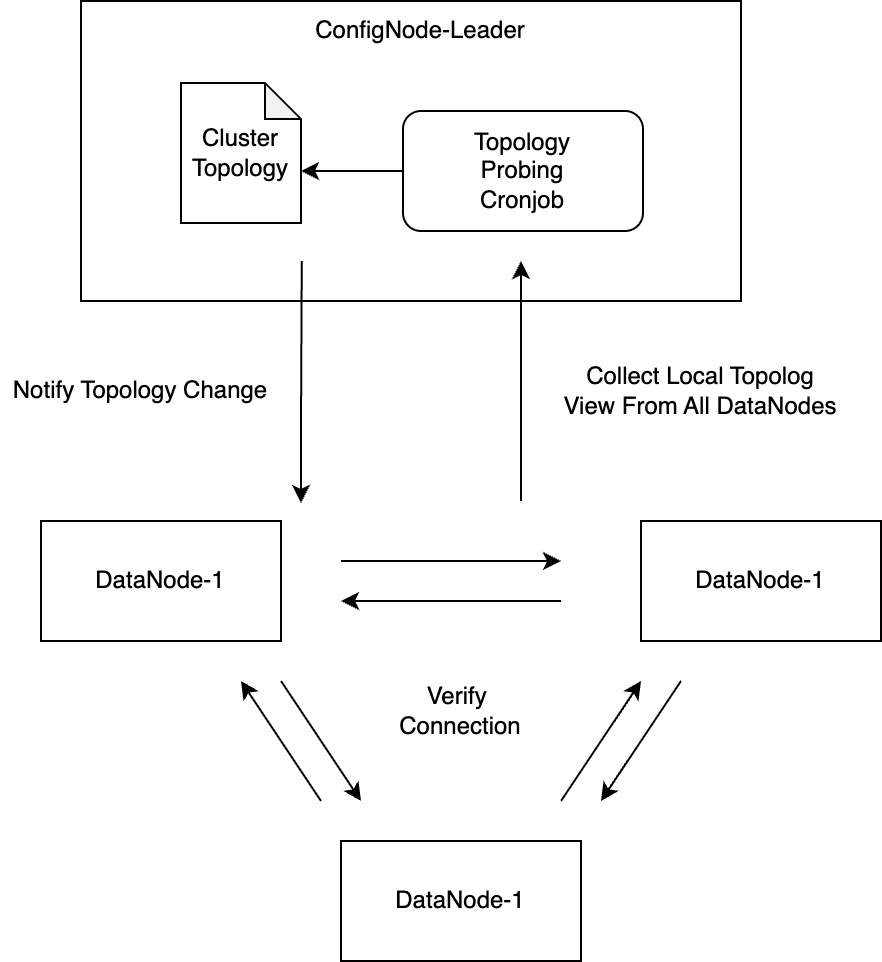
\includegraphics[width=0.7\linewidth]{c03-topology.png}
  \caption{集群拓扑感知能力}
  \label{fig:c03-topology}
\end{figure}

我们通过DataNode之间的P2P心跳来实现集群拓扑感知的功能。图\ref{fig:c03-topology}展示了集群拓扑感知的全流程。ConfigNode Leader会启动定期的任务,要求每一个DataNode需要向其他的所有DataNodes发送探测性质的RPC请求,来验证是否能够和所有DataNodes都完全联通,并在规定的时间内向ConfigNode上报本次的探测结果。

ConfigNode会收集所有DataNode的本地连通性,并同样维护一个固定大小的采样窗口。接着ConfigNode会使用上一小节中提到的Phi Accrual算法来判断DataNodes之间的两两连通性,最终获得全局拓扑图。
一旦ConfigNode发现全局拓扑图更新,那么就会在下一次和DataNode交换心跳包的时候将这个拓扑图给下发到每一个DataNode节点,使得每一个DataNode节点上都能够存储一份最新的集群视角的拓扑结构,用于后续的查询计划生成和写入请求。


\section{基于长期连接的优化}

在部分情况下,例如通过操作系统强制Kill一个IoTDB进程,我们可以通过特殊的机制进一步加快错误的发生,这是通过TCP信道来实现的。
IoTDB内部采用ClientManager接口来统一管理对外的Thrift连接。ClientManager的基本原理类似于带缓存的连接池。当我们首次请求某一个新的EndPoint的TCP连接请求,ClientManager会建立这个TCP连接。当我们结束使用的时候,ClientManager并不会直接将这个TCP连接断开,而是继续维持一段时间,并把连接缓存在本地。这样在下次我们需要请求相同的EndPoint地址的时候,我们就不需要负担重新建立TCP的开销,可以直接复用ClientManager内部缓存的连接。当我们长期不使用某一个TCP连接的时候,ClientManager就会销毁这个连接并且清理对应的资源。

由于ConfigNode和每一个DataNode之间都有大量的内部RPC交换,因此通过ClientManager的机制,我们可以认为ConfigNode和DataNode之间建立了一个长期有效的TCP连接信道。此时当该进程突然断开,那么Thrift就能够立马汇报信道的问题,这种汇报的时间延迟通常在一秒钟之内,非常快速,而不需要依赖上述所说的Phi Accural算法,后者的发现延迟通常在十秒之上。


(其实这里我觉得应该变成Thrift连接)


\section{基于集群实时监控的检测}

IoTDB通过建设了较为完整的可观测性,从而进一步提升集群快速、准确发现故障的能力,显著提升了故障诊断和问题排查的能力。

可观测性不仅是监控的延伸,更是一种深入理解系统内部状态和行为的方法论。它通过收集和分析Metrics(指标)、Logging(日志)和Tracing(追踪)等多维度的数据,帮助运维人员全面掌握系统的运行状况,从而实现更高效的故障发现和解决。

可观测性是指通过系统的外部输出,推断其内部状态的能力。与传统的监控不同,可观测性强调对系统行为的深层次理解,而不仅仅是关注预定义的指标。在分布式系统中,由于组件之间的复杂交互和依赖关系,故障的根源往往难以追踪。可观测性通过提供多维度的数据,帮助运维人员从全局视角理解系统行为,快速定位故障根源。

可观测性对于故障发现的意义主要体现在以下几个方面:

早期预警: 通过实时监控Metrics指标,可以及时发现系统的异常行为,如CPU使用率过高、内存泄漏等,从而实现早期预警。
快速定位: 通过分析Logging日志和Tracing追踪数据,可以追踪请求的完整生命周期,了解请求在各个组件之间的流转情况,快速定位故障发生的具体位置。
根因分析: 通过综合分析Metrics、Logging和Tracing数据,可以深入了解故障的根本原因,为问题解决提供有力支持。
性能优化: 可观测性不仅可以用于故障发现,还可以帮助运维人员了解系统的性能瓶颈,从而进行针对性的优化。


Metrics、Logging和Tracing的介绍

Metrics(指标):
Metrics是量化的度量,用于描述系统的运行状态。例如,CPU使用率、内存使用率、请求响应时间等。
IoTDB通过内置的Prometheus reporter,将各个节点的Metrics数据暴露给Prometheus进行采集,并通过Grafana面板进行可视化展示。
通过监控Metrics指标,运维人员可以实时了解系统的运行状况,及时发现异常行为。
Logging(日志):
Logging是记录系统运行过程中发生的事件和错误信息。
IoTDB的Logging日志包含了详细的系统运行信息,如请求处理过程、错误信息等。
通过分析Logging日志,运维人员可以了解系统内部的运行细节,追踪错误发生的轨迹。
Tracing(追踪):
Tracing是追踪请求在分布式系统中的完整生命周期。
通过Tracing,运维人员可以了解请求在各个组件之间的流转情况,分析请求的性能瓶颈。
Tracing对于分布式系统中的性能分析和故障诊断具有重要意义。

\begin{figure}
  \centering
  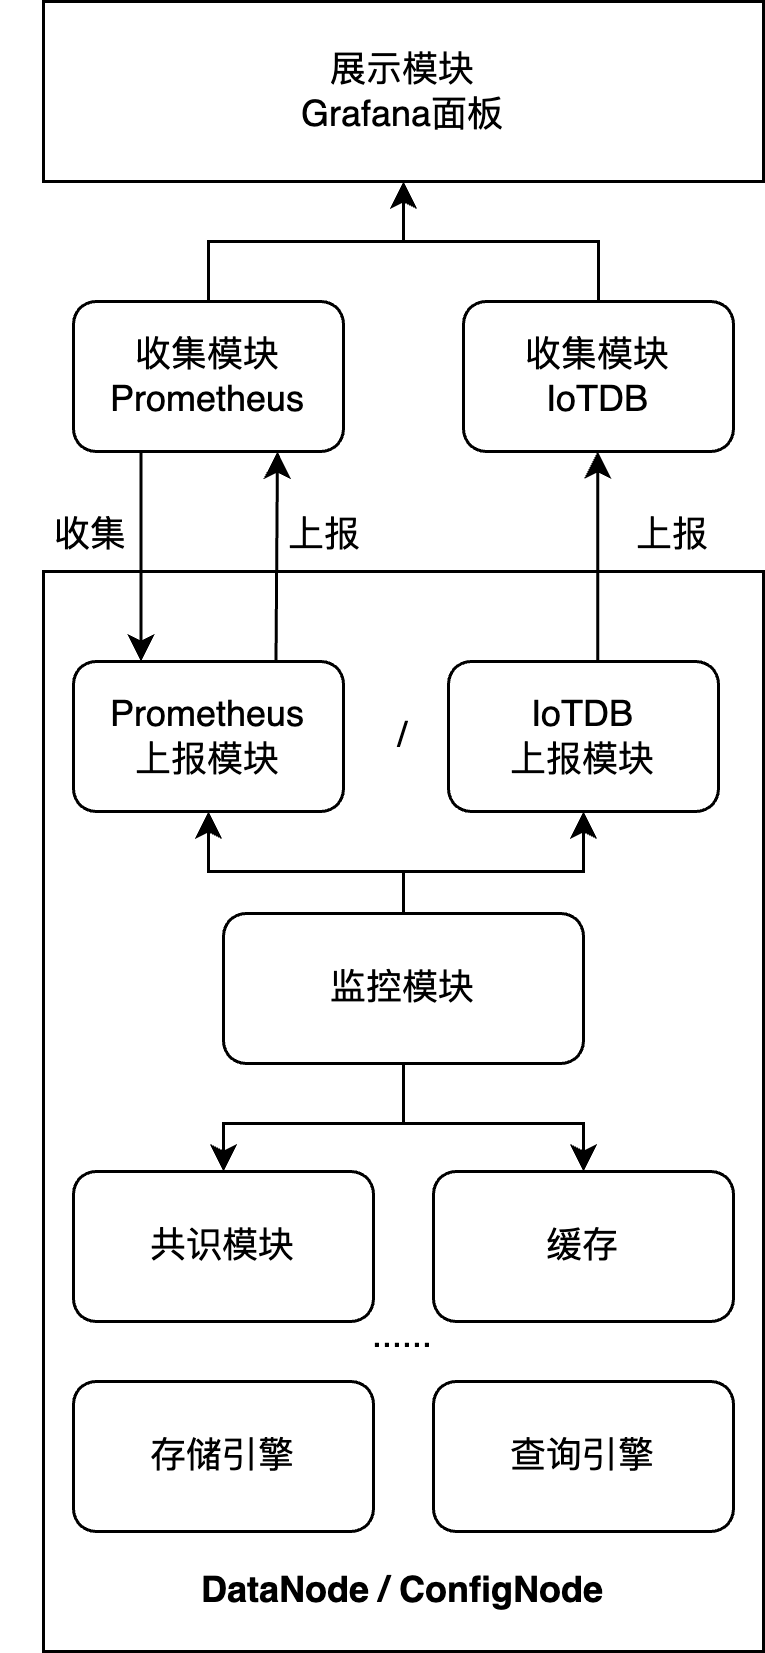
\includegraphics[width=0.4\linewidth]{c03-metrics-arch.png}
  \caption{集群拓扑感知能力}
  \label{fig:c03-metrics-arch}
\end{figure}

图\ref{fig:c03-metrics-arch}给出了IoTDB可观测性的监控建设的架构图。IoTDB内部通过实现通用的监控模块服务,来实现统一的监控接口,来隔离不同的采集程序的接口和IoTDB不同模块之间的差异。
每一个模块都会调用监控服务提供的接口,注册并上报自身的相关重要数据,例如内存使用情况、关键路径上的性能指标等。

监控最终会被外部程序采集,例如,会被存储到Prometheus上,甚至是别的IoTDB实例当中。根据外部存储的不同,IoTDB在启动的时候会根据配置加载对应的上报模块。
在每一个DataNode和ConfigNode内部都有上报模块,负责将监控模块收集到的数据定期上报到外部存储中。目前上报模块支持两种不同的采集方式,一种是拉取,例如普罗米修斯,会定期向节点中的reporter拉取数据。还有一种是主动的推送模式,例如IoTDB。



这里应该给出IoTDB的监控模块的实现
(包括所有的采集指标)
- CPU:CPU 核数,利用率等
- 磁盘:带宽,IOPS 等
- 网络:发送速度,接收速度,TCP 连接数等
- JVM:
  - 线程
    - JVM 当前线程数
    - 当前 daemon 线程数
    - 峰值线程数
    - 当前处于各种状态的线程数
  - 垃圾回收
    - YGC、FGC 发生次数与原因
    - YGC、FGC 累计耗时与原因
    - YGC、FGC 最大耗时与原因
    - GC 消耗 CPU 的比例
    - 从 GC 之前到 GC 之后老年代内存池大小正增长的累计
    - 老年代内存的历史最大值
    - GC 之后老年代内存的大小
    - 在一个 GC 之后到下一个 GC 之前年轻代增加的内存
  - 内存
    - 已经使用的缓冲区大小
    - 最大缓冲区大小
    - 当前缓冲区数量
    - 当前向 JVM 申请的内存大小
    - JVM 最大内存
    - JVM 已使用内存大小
  - Classes
    - JVM 累计卸载的 class 数量
    - JVM 累计加载的 class 数量
    - JVM 消耗在编译上的时间